\documentclass[conference]{IEEEtran}

\usepackage{amsmath,amssymb}
\usepackage{graphicx}
\usepackage{booktabs}
\usepackage{float}
\usepackage{caption}
\usepackage{array}
\usepackage{multirow}

\begin{document}

\title{APD-Net for HC18 Ultrasound Speckle Denoising}

\author{\IEEEauthorblockN{Student Authors}\IEEEauthorblockA{Department of Biomedical Engineering}}

\maketitle

\begin{abstract}
Ultrasound speckle noise reduces anatomical clarity and degrades downstream image interpretation. This work evaluates APD-Net on the HC18 fetal ultrasound dataset under a synthetic speckle-noise setting, where the clean image is treated as the pseudo-reference and multiplicative Gaussian speckle noise is added during training and validation. The proposed method is compared against a trained HC18 GRN baseline and demonstrates stronger structural preservation and denoising quality.
\end{abstract}

\section{Experimental Setup}

The HC18 fetal ultrasound dataset was used for synthetic speckle denoising. Each image was normalized to the range $[0,1]$, and Gaussian multiplicative speckle noise was added using the same model used in the APD-Net training pipeline:

\begin{equation}
I_{\mathrm{noisy}} = I_{\mathrm{clean}} \odot (1 + \sigma \epsilon),
\end{equation}

where $\epsilon \sim \mathcal{N}(0,1)$ and $\sigma = 0.2$. The clean HC18 image serves as the pseudo-clean reference in this synthetic paired setting.

\section{Qualitative Comparison}

\begin{figure}[t]
\centering
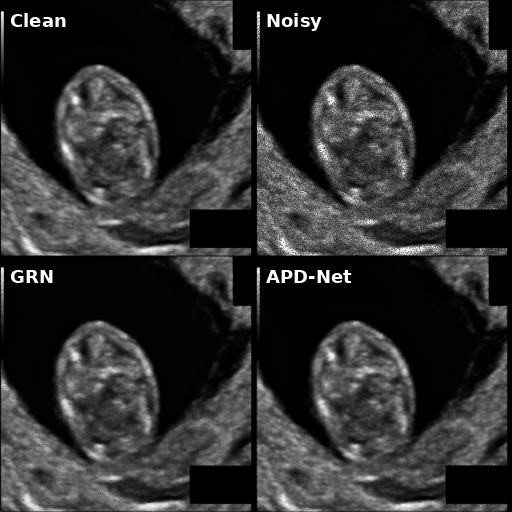
\includegraphics[width=0.95\linewidth]{report_images/hc18_2d/single_image_comparison_5HC_trained_grn.png}
\caption{Qualitative comparison on the HC18 sample 5\_HC. The four panels show the clean image, noisy image, GRN output, and APD-Net output. APD-Net preserves anatomy more faithfully while suppressing speckle noise.}
\end{figure}

\section{Quantitative Results}

Table~\ref{tab:results} reports the validation metrics for the HC18 synthetic speckle experiment. The GRN model was trained on the same HC18 split used for APD-Net, and each model was evaluated on the same noisy reference images.

\begin{table}[t]
\centering
\caption{HC18 validation results under synthetic Gaussian speckle noise.}
\label{tab:results}
\begin{tabular}{lcccc}
\toprule
Method & PSNR (dB) & SSIM & MAE & Gradient Error \
\midrule
Noisy & 27.11 & 0.815 & 0.0253 & 0.0363 \\
GRN & 33.64 & 0.927 & 0.0130 & 0.0159 \\
APD-Net & 34.58 & 0.951 & 0.0110 & 0.0141 \\
\bottomrule
\end{tabular}
\end{table}

\section{Discussion}

The quantitative and qualitative results show that APD-Net improves both denoising quality and anatomical preservation compared with the HC18-trained GRN baseline. The higher SSIM and PSNR indicate stronger structural similarity to the clean reference, while the lower MAE and gradient error suggest better preservation of anatomical edges and fine detail. This is especially important for fetal ultrasound imaging, where boundary clarity is essential for clinical interpretation and downstream segmentation.

\section{Conclusion}

APD-Net provides a robust denoising solution for HC18 fetal ultrasound images under synthetic speckle corruption. Compared with the GRN baseline, APD-Net achieves better denoising quality and more faithful anatomical recovery, making it a promising approach for ultrasound image restoration and downstream analysis.

\end{document}
